\documentclass{article}
\usepackage{graphicx} %package to manage images
\graphicspath{ {./images/} }
\usepackage[rightcaption]{sidecap}
\usepackage{wrapfig}




\begin{document}

\begin{titlepage}

  \centering
  {\Large \bfseries  E-Commerce site(Scroll through)}
  \vspace{6\baselineskip}
  
  
  
  
  {\Large \bfseries \underline{Course}\\ \vspace{0.5\baselineskip} Technical Writing and Presentation}
  \vspace{5\baselineskip}
  
  
  
  
  {\Large \bfseries \underline{Submitted to}\\ \vspace{0.5\baselineskip} Dr. Ahsan Habib \\ \vspace{0.4\baselineskip}
   Assistant Professor, IICT, SUST}
  \vspace{5\baselineskip}
  
 
 
  
  {\Large \bfseries \underline{Submitted by}\\ \vspace{0.5\baselineskip}Shreshthajit Das(2017831013) \\ \vspace{0.4\baselineskip}
   Md. Ismail Hosen(2017831061)}
  \vspace{5\baselineskip}
 
 

   
  {\Large \bfseries \underline{Submission Date}\\ \vspace{0.5\baselineskip}22 February 2021}
  \vspace{3\baselineskip}
 
\end{titlepage}




















\tableofcontents

\newpage
%\chapter{Document}
%\chapter{Nothing}
%\chapter{Client Brief}
%\chapter{Objective}
%\chapter{Scope Of Work}
%\chapter{Administrative Panel}
%\chapter{Requirements From Clients}
 

\section{Project Description}

\subsection{Project overview}
E commerce is fast gaining ground as an accepted and used \\ business
paradigm.More and more business houses are implementing web sites
providing functionality for performing commercial transactions over the web. It is reasonable to say that the process of shopping on the web is becoming common place.In our website an admin can sell electornic accessories like mobile,watch,laptop etc.

\subsection{Purpose of the Project}
\subsubsection{Background of the Project Effort}
The objective of this project is to develop a general purpose e-commerce store where electronic accessories   can be bought from the comfort of home through the internet. However, for implementation purposes, this paper will deal with an online shopping for Electronic accessories.
\subsubsection{ Goals of the Project}
An online store is a virtual store on the Internet where customers can browse the catalog and select products of interest. The selected items may be collected in a shopping cart. At checkout time,the items in the shopping cart will be presented as an order. At that time more information will be needed to complete the transaction. Usually , the customer will be asked to fill or select a billing address, a shipping address, a shipping option, and payment information such as bKash, or Cash on delivery. An e-mail notification is sent to the customer as soon as the order is placed.
\subsection{The Scope of Work}
With the developing utilization of media machines like a Smartphone, workstation, PC with web access, the skyline of e-commerce business improvement is extending day-by-day. Due to the accessibility of contraptions and simple web access has lead individuals to web-based shopping. Among many, expanding the tech-mindful populace, web speed and availability mediums are the most compelling variables for e-commerce business advancement on the planet.




\subsection{Stakeholders}
\begin{tabular}{ |p{4cm}|p{4cm}|}
% \hline
 %\multicolumn{2}{|c|}{Country List} \\
 \hline
 User Category & User Actions\\
 \hline
 
 

Admin & 
1.Create
2.Delete
3.Update product
4.Add\\
 \hline
 
 Customer &
 1.Add item to his cart
 2.Delete Unnecessary item from cart
 3.Edit item count

 \\

\hline
\end{tabular}



 
 
 
 
 \section{System Analysis}
 Feasibility Study:A feasibility study examines the practicability of an idea, a project or even a new business.The objective of feasibility study is to place an accentuation on latent issues that could befall if the project is sought after and decide whether, after every substantial factor are taken into account, the project should be pursued or not. It enables organizations to determine all of the obligatory details to make a business prosperous. A feasibility study distinguishes strategic issues, and almost all business-related issues, alongside providing answers to lighten them. The operational (will it work?), economical (cost and benefits) and technical (can it be built?) aspects are part of the study.
 
    • Operational Feasibility
    • Technical Feasibility
    • Economic Feasibility
    • Schedule Feasibility

 

\subsection{Operational Feasibility}
The  Operational  feasibility  evaluation  concentrates   on  how  much  the  proposed
advancement project fits  in with the current institute condition and targets concerning
improvement plan, ease the learning process and keep the students up to date.To guarantee achievement, desired operational results must be conveyed during design and development. These incorporate such outline subordinate parameters as reliability, maintainability, supportability, usability, disposability, sustainability, affordability and others.
Here in our Department Collaboration system since the student ,teachers also admins are enough educated so we think it possible to incorporate the outlines of the operational parameters.

\subsection{Technical Feasibility}
Technical feasibility is a procedure of determining if the organization has the innovation
assets to create or buy, introduce, and operate the system. Does the organization have the
mechanical assets to embrace the venture?
It is highly feasible for this organization to continue this system.Technical requirements are easy to fulfil.All are available at the hand. We also suggest contacting a hosting company to take necessary steps to host this system.

\subsection{Economic Feasibility}

System development and yearly working expenses are the two essential segments used to decide the cost gauges for a proposed information system.Since this system is developed for our course so there no

expense for development.The Yearly working expenses are the hosting charge ,maintenance and other charges.According to the cost scenario the system is feasible.

\subsection{Schedule Feasibility}
As indicated by Shelly Cashman (2010), schedule feasibility can be characterized as, the way toward deciding if a venture can be executed inside a given time allotment in connection to the organizational due dates and constraints. Fundamentally, it is the way toward dissecting the time period  as to when the  venture  might  be  finished. This  possibility  covers  how  the assignments should be partitioned and the measure of time therefore utilized for the  effective culmination of the venture.

\newpage

\section{Detailed System Description}

\subsection{Client Brief}
Client desires to develop an e-commerce website.\\
\\
a)Customer will be able to login/register into the website.\\
b)Customer will be able to creating an account after submitting
their email id,name,address etc on the website.\\
c)Customer will be able to easily search for products by using
different keywords like name,category wise etc and will be able to
refine their results by using filters such as price,product types etc
on the website.\\
d)Customer will be able to view the products with
details,images,zoom in option etc on the website.\\
e)Customer will be able to customize their products by submitting
the information on the website.\\
f)Customer can view the events posted by the admin on the
website.7)Customer can submit their views on the products listed on the
website.\\
g)Customer will be able to place orders on the website.
h)Customer will be able to check their order status on the website.\\
i)Customer will be able to make payments for their orders by
using integrated payments system.\\
j)Customer will be able to view the shipping details on the
website.\\
k)Customer will be able to view the FAQ on the website.\\


\subsection{User visibility content}
-Information bar.\\
-Menu bar.\\
-Tool bar.\\
-Side bar.\\
-Header.\\
-Footer.\\
-Text and Graphics.\\


\subsection{Design Specifications}
The design and layout application will be constructed using
CSS,HTML,PHP along with use of AJAX and keeping in mind
latest web trends.
\\

\subsection{Front End}
The Front end will have the following features:\\
-Home\\
-Login/Sign-up\\
-Search\\
-About us\\


\subsection{Footer Page}
-Contact us\\
-Sitemap\\
-Terms and Conditions\\
-Privacy policy\\
-FAQ\\






\subsection{Website Content Page}
-Home\\
-My account control panel for customers\\
-Search Advanced search\\
-Products\\
-Product\\
-Product Catalog\\
-Products Information\\
-Customize\\
-Reviews\\
-Events\\
-Shopping Cart\\
-Checkout\\
-Shipping\\
-Payments\\
-Social Media Integration\\
-Newsletter\\
-Contact us\\

\subsection{Hardware needs for e-commerce}
Hardware needs for e-commerce
Hardware requirements for high traffic sites may depend on the following factors: the number of transactions per second; Hits per second; Number of questions per second; Number of queries completed by RDBMS per second; The page number is served per second associated with the parameters mentioned above.
Some other elements that may be considered when setting up high traffic e-commerce sites include clustering, such as backup servers that handle operations automatically when initially fail without filling out the proper ecommerce website development requirements.

\section{ User Interface Specification
}

\subsection{Customer Registration}
This is the section where customer will be able to register to the
site as member. Once customer shows interest and wants to get an
account then he will be taken to a page where he will be
asked to submit a form that would have various fields for the
customer to enter their personal details creating a profile of their
own.\\

\subsection{Existing Customer}
After the account is being activated customer will be able to
perform the following basic tasks in account setting:\\
a)Customer would be able to login.\\
b)Customer would be able to view their account after successful
login.\\
c)Customer would be able to add/edit/delete all their details.\\

\section{Function of customer}
-Customer will be able to login/register into the website.\\
-Customer will be able to create account after submitting their
email id,name,address on the website.\\
-Customer will be able to easily search for products by using
different keywords category wise etc.\\
-Customer would be able to view their account after successful
login.\\



\subsection{Product}
Products will be sorted according to the categorywise and
subcategory wise. Once a category is selected all the list will come
out along with the image and other necessary details. If a customer
clicks into a products he will be taken to a page where the
complete details about the product is listed.\\


\subsection{Shopping Cart}
The shopping cart will allow the customers to manage their
shopping in an easy and convenient way. The shopping cart will
carry the following features:\\
-Customer can view their order history and order status.\\
-All order will be stored in the database for fast efficient retrieval.\\
-Temporary shopping cart for guests and permanent cart for
customers.\\
-Add updates in real time.\\
-Full product stock control.\\
-Payment options.\\
-Shipping and billing address.\\
-Recalculate the total value.\\





\section{Administrative Panel}
The back end of the website will be powerplaned with an
administrative panel to manage the updation of data at the front as
well as back end.Following are the key functions\\
-Customer management\\
-Product management\\
-General management\\
-Order management\\
-Content management\\
-Reports management\\


\subsection{Customer Management}
 
→Admin will be able to manage the customer of the website\\
→Admin will be able to add/delete customers of the website\\
→ Admin will be able to approve/reject the registration of the
customer.\\
→ Admin will be able to view the list of customers in the website.\\
→ Admin will be able to activate/deactive the customers on the
site.\\

\subsection{Product management}
→ Admin will be able to manage the categories and sub categories.\\
of products on the website.
→ Admin will be able to add/delete.\\


\subsection{General Management}
 
→ Manage shipping.\\
→ Manage reviews.\\
→ Manage events.\\
→ Manage inventory.\\

\subsection{Order Management}
 
→ Admin can manage the order received by the website.\\
→ Admin can add/delete orders received by the website.\\
→ Admin can search the orders received by the website.\\
→ Admin can view the list of all orders received by the site.\\
→List of customers.\\
→ Payment reports.\\
→Sales Reports.\\
→ Inventory Reports.\\
















\subsection{Content Management}
Admin will be able to add/delete text/images/videos of the items
on the site.The admin will be provided a rich interface editor
which will enable him to create as many pages as required .Admin
will be able to add text,images,links etc to the pages and those
pages can be liked to any other pages on the same site.
\\
 


















\section{Diagrams}
\subsection{Context Diagram}
The Context Diagram shows the system under consideration as a single high-level process and then shows the relationship that the system has with other external entities (systems, organizational groups, external data stores, etc.). 
\\
\\
\vspace{5\baselineskip}
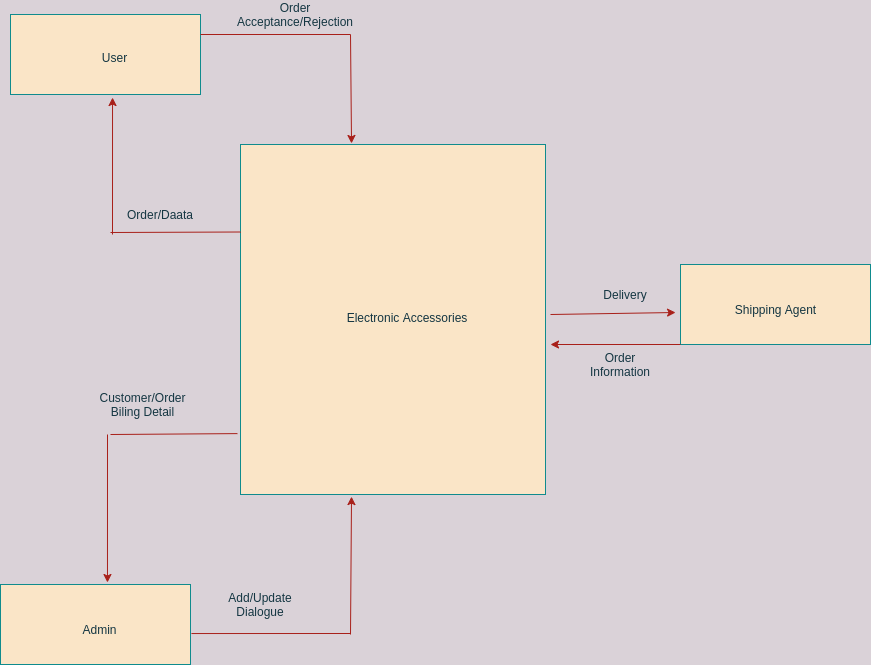
\includegraphics[width=12cm]{images/context_dia.png}

























\subsection{Use Case Diagram}
A UML use case diagram is the primary form of system/software requirements for a new software program underdeveloped. Use cases specify the expected behavior (what), and not the exact method of making it happen (how).A key concept of use case modeling is that it helps us design a system from the end user's perspective. It is an effective technique for communicating system behavior in the user's terms by specifying all externally visible system behavior.
 \\
\\
\vspace{5\baselineskip}
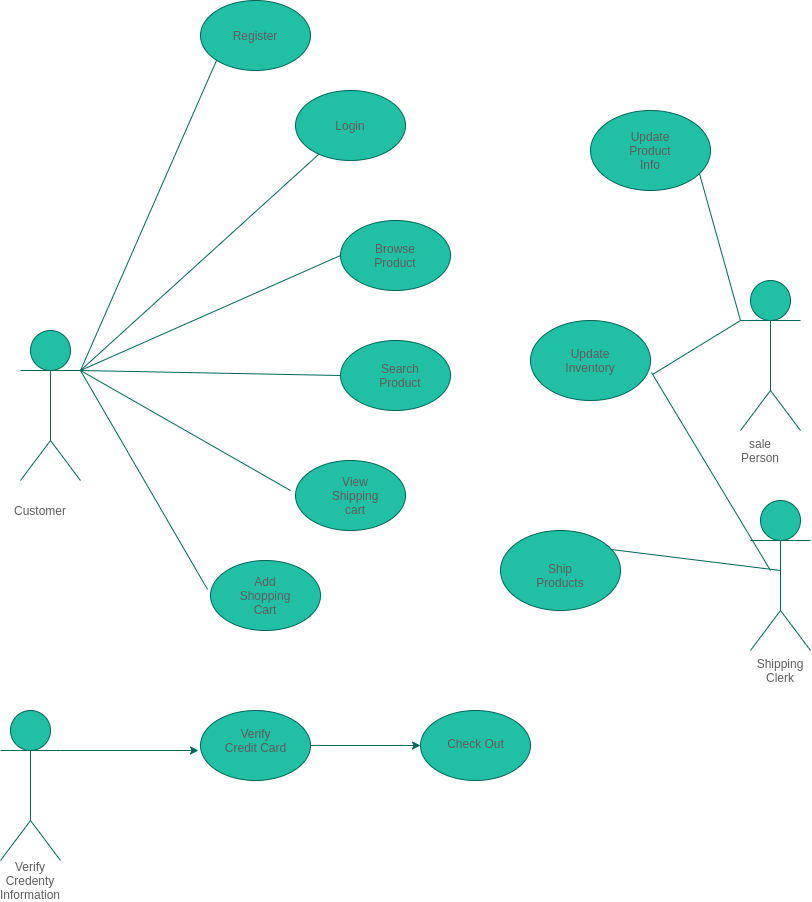
\includegraphics[width=12cm]{images/use_case.png}




























\subsection{Data Flow Diagram}
Label:1(Add User)

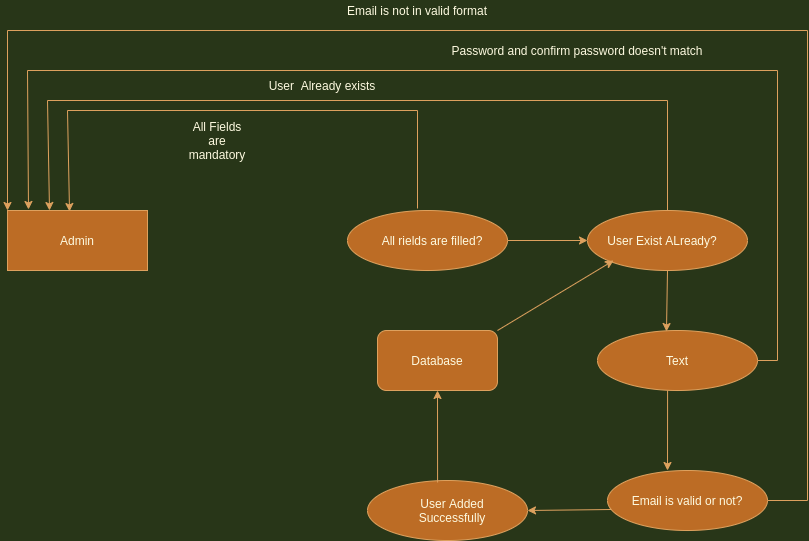
\includegraphics[width=12cm]{flow}
 \vspace{10\baselineskip}
 
Label:2(Resolve Issues)
 
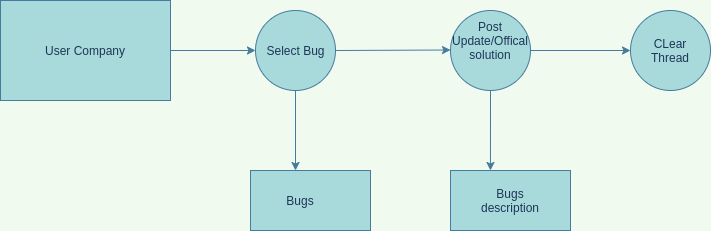
\includegraphics[width=12cm]{images/Resolve_issues.png}
\newpage


Label:3(Report bug)
\\
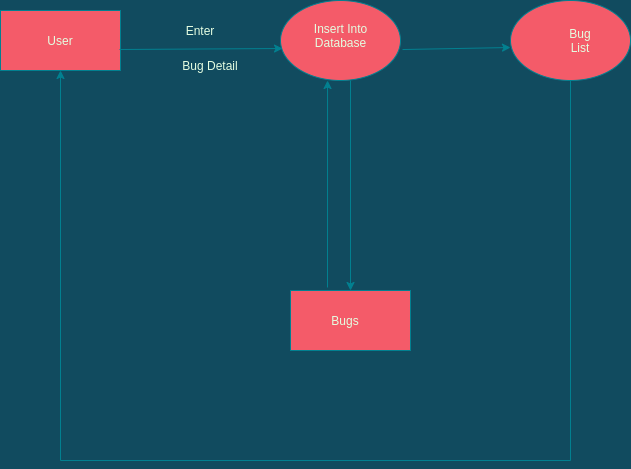
\includegraphics[width=12cm]{images/Report_bug.png}

\vspace{2\baselineskip}
 Label:4(Provide Solution)
 \\
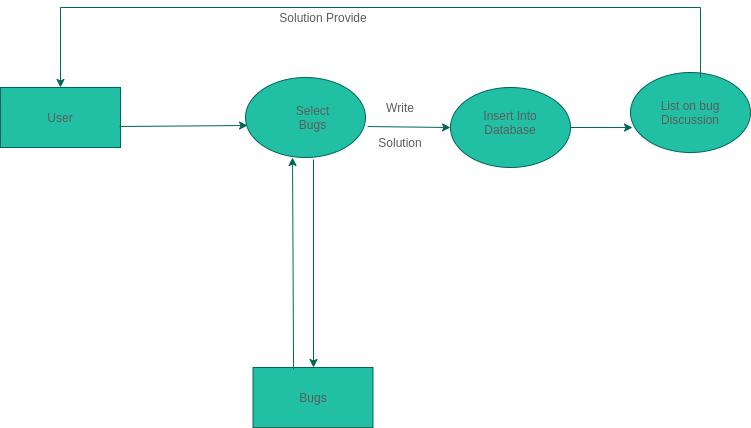
\includegraphics[width=10cm]{images/bug_solution.png}
\vspace{4\baselineskip}
\\
\\
\\
\\
\\


















\section{Requirements From Client}
This website require the following from client.This information
would be solely used for the project purpose.\\
→ Detailed document in case anymore features need to be added
on the website.\\
→ Point of contact to discuss the updates on a daily or a weekly
basis as prefered by client.\\
→ Details like address ,name,telephone numbers ,website,photos
etc pertaining to all the categories mentioned in the methodology.\\
→ Focus on User Experience.\\

\subsection{Buyer Reviews}
Want to hear from real people to see if the products fit their desires and expectations about their product experience. According to Kissmetrics, 55  of buyers say that online review affects their buying decision by optimizing functional requirements for e commerce website.
 

Statistica reported that 17 of customers abandoned online shopping carts due to concerns about payment protection. Strong assurance for tired buyers to post a security and certification symbol from respected third party security agencies.
 
Build trust with your customers by posting customer product reviews on your site. And if positive reviews are helpful, do not be afraid to post negative reviews – your transparency creates reliability on your brand’s integrity.
\subsection{Security mark}
Remove customer fear with evidence that their information is safe and secure. ecommerce website security requirements are one of the top priorities.

\vspace{5\baselineskip}

\section{Conclusion}
After careful observation, it has come to my conclusion that e-commerce has undeniably become an important part of our society. The world wide web is and will have a large part in our daily lives. It is therefore critical that small businesses have their own to keep in competition with the larger websites. Since web developers have lowered down the prices for their services, it has become more affordable for small businesses to use the world wide web to sell their products. Although there are negative aspects of e-commerce, small businesses have tried to accommodate to the needs of the consumers. For example, one of the negative aspects of e-commerce is that consumers lack the advice and guidance of sellers, to accommodate that, they have customer service through the phone of online to answer any questions. It is also important to note that e-commerce does not benefit all small companies equally. How much revenue a business gets from e-commerce depends on what kind of service it gives. For example, most people would like to try on clothes before they buy them, so it probably would not benefit a small business that sells clothes as much as a small business that sells home supplies or specialty books. Nevertheless, e-commerce does benefit any business even in small ways. This is why it is crucial to understand how e-commerce affects small businesses because it is becoming such a huge part of how society functions that it effects the economy greatly and whatever happens to the economy affects us. This is why is it important to understand this subject because in the long run, it will affect all of us.



 



\end{document}


